\documentclass[11pt]{article}
\usepackage[utf8]{inputenc}
\usepackage{amsmath,amsthm,amsfonts,amssymb,amscd}
\usepackage{multirow,booktabs}
\usepackage[table]{xcolor}
\usepackage{fullpage}
\usepackage{cancel}
\usepackage{lastpage}
\usepackage{physics}
\usepackage{enumitem}
\usepackage{fancyhdr}
\usepackage{simpler-wick}
\usepackage{mathrsfs}

\usepackage{wrapfig}
\usepackage{tikz}
\usepackage{tikz-feynman}
\usepackage{setspace}
\usepackage{calc}
\usepackage{multicol}
\usepackage{cancel}
\usepackage[retainorgcmds]{IEEEtrantools}
\usepackage[margin=3cm]{geometry}
\usepackage{amsmath}
\newlength{\tabcont}
\setlength{\parindent}{0.0in}
\setlength{\parskip}{0.05in}
\usepackage{empheq}
\usepackage{framed}
\usepackage[most]{tcolorbox}
\usepackage{xcolor}
\usepackage{tcolorbox}
\usepackage{slashed}
\usepackage{dsfont}
\colorlet{shadecolor}{orange!15}
\parindent 0in
\parskip 12pt
\geometry{margin=1in, headsep=0.25in}
\theoremstyle{definition}
\newtheorem{defn}{Definition}
\newtheorem{reg}{Rule}
\newtheorem{exer}{Exercise}
\newtheorem{note}{Note}
\usetikzlibrary{arrows.meta}
\usetikzlibrary{patterns.meta, positioning, shapes.geometric}
\allowdisplaybreaks[4]
\usepackage[utf8]{inputenc}
\usepackage{titlesec}

\usepackage[colorlinks=true, linkcolor=blue, urlcolor=blue, citecolor=blue]{hyperref}

\usepackage{tikz}
\usepackage{tikz-feynman}

\geometry{tmargin=.75in, bmargin=.75in, lmargin=.75in, rmargin = .75in}  

\newcommand{\R}{\mathbb{R}}
\newcommand{\C}{\mathbb{C}}
\newcommand{\Z}{\mathbb{Z}}
\newcommand{\N}{\mathbb{N}}
\newcommand{\Q}{\mathbb{Q}}
\newcommand{\A}{\mathcal{A}}
\newcommand{\Lagrangian}{\mathcal{L}}
\newcommand{\Cdot}{\boldsymbol{\cdot}}

\newtheorem{thm}{Theorem}
\newtheorem{conv}{Convention}
\newtheorem{rem}{Remark}
\newtheorem{lem}{Lemma}
\newtheorem{cor}{Corollary}
\newtheorem{ex}{Exercise}


\title{Peskin Solutions}
\author{Luca Jin}
\date{2025}

\begin{document}

\maketitle
\tableofcontents

\vspace{.25in}

\section{Chapter 6}
\subsection{6.2 Equivalent Photon Approximation}
Consider the process in which electrons of very high energy scatter from a target. In leading order in $\alpha$, the electron is connected to the target by one photon propagator:
\vspace{.4in}
\begin{equation}
    i\mathcal{M} =
    {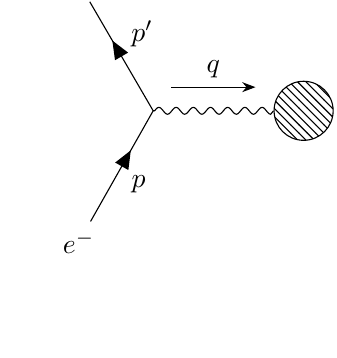
\begin{tikzpicture}[baseline={(0,-0.85)}]
    \feynmandiagram [horizontal=a to b] {
    i1 [particle=\(e^{-}\)] -- [anti fermion, edge label = $p'$] a -- [anti fermion, edge label = $p$] i2 [particle=\(e^{-}\)],
    a -- [photon, momentum=\(q\)] b [blob],
    };            
    \end{tikzpicture}}
\end{equation}
where the blob is, in general, complicated coupling of the virtual photon to the target.

If the initial and final energies of the electron are $E$ and $E'$. Under the high-energy limit, 
\begin{equation}
    p = (E, 0,0,E), \quad p'=(E',E'\sin\theta,0,E'\cos\theta),
\end{equation}
which implies
\begin{equation}
    q^2 = (p'-p)^2 = -2EE'(1-\cos\theta).
\end{equation}
In the limit of forward scattering, whatever the energy loss, the photon momentum approaches $q^2 = 0$; thus the reaction is highly peaked in the forward direction. It is tempting to guess that, in this limit, the virtual photon becomes a real photon. Let us investigate in what sense that is true.

\textbf{(a)} The matrix element of the above process is given by
\begin{equation}
    \mathcal{M} = (-ie)\bar{u}(p')\gamma^\mu u(p)\frac{-ig_{\mu\nu}}{q^2}\hat{\mathcal{M}}^\nu(q),
\end{equation}
where $\hat{\mathcal{M}}^\nu(q)$ represents the (in general, complicated) coupling of the virtual photon to the target. Let us analyse the structure of the piece $\bar{u}(p')\gamma^\mu u(p)$. Let $q = (q^0,\vec{q})$ and $\Tilde{q}=(q^0,-\vec{q})$. We can expand the spinor products as 
\begin{equation}
    \bar{u}(p')\gamma^\mu u(p) = Aq^\mu + B\Tilde{q}^\mu + C \epsilon_1^\mu + D\epsilon_2^\mu,
\end{equation}
where $A, B, C , D$ are functions of the scattering angle and energy loss and $\epsilon_1, \epsilon_2$ are two unit vectors transverse to $\vec{q}$. By dotting the expression with $q^\mu$, we find
\begin{equation}
    q_\mu \cdot [\bar{u}(p')\gamma^\mu u(p)] = Aq^2 + Bq\cdot \Tilde{q}.
\end{equation}
By Ward identity, we have $q_\mu \bar{u}(p')\gamma^\mu u(p)]=0$. Thus, we have
\begin{equation}
    B = -A\frac{q^2}{q\cdot \Tilde{q}} \approx A \frac{2EE'(1-\cos\theta)}{(q^0)^2 + \vec{q}^2} \sim \theta^2.
\end{equation}
Thus, $B$ can be ignored in the case of forward scattering.

Again, by Ward identity, we have $q\cdot \hat{\mathcal{M}}(q) = 0$. Thus, $A$ can be ignored as well.

\textbf{(b)} In the frame where $p=(E,0,0,E)$, the spinor $u_s(p)$ is given by 
\begin{equation}
    u_s(p) = \begin{pmatrix}
        \sqrt{p\cdot \sigma}\xi_s\\
        \sqrt{p\cdot \bar{\sigma}}\xi_s,
    \end{pmatrix}
\end{equation}
where
\begin{equation}
    \sigma^3\xi_\pm = \pm\xi_\pm \implies \xi_+ = \begin{pmatrix}
        1\\0
    \end{pmatrix}, \quad \xi_-=\begin{pmatrix}
        0\\1
    \end{pmatrix},
\end{equation}
and
\begin{equation}
    \sqrt{p\cdot \sigma} = \sqrt{E(1 - \sigma^3)}, \quad \sqrt{p\cdot \sigma} = \sqrt{E(1 + \sigma^3)}.
\end{equation}
Thus,
\begin{equation}\boxed{
    u_+(p) = \sqrt{2E}\begin{pmatrix}
        0\\0\\1\\0
    \end{pmatrix},\quad u_-(p)=\begin{pmatrix}
        0\\1\\0\\0
    \end{pmatrix}.}
\end{equation}

Next, let us evaluate $u(p')$. Using $p' = (E', E'\sin\theta,0,E'\cos\theta)$, we find
\begin{equation}
    \hat{p}'\cdot \vec{\sigma} \xi_\pm = \pm \xi_\pm \implies \xi_+ = \begin{pmatrix}
        \cos\frac{\theta}{2}\\\sin\frac{\theta}{2}
    \end{pmatrix},\quad \xi_- = \sqrt{2E}\begin{pmatrix}
        -\sin\frac{\theta}{2}\\\cos\frac{\theta}{2}
    \end{pmatrix}
\end{equation}
and
\begin{equation}
    \sqrt{p\cdot \sigma} = \sqrt{E'(1-\hat{p}\cdot \vec{\sigma})}, \quad \sqrt{p\cdot \bar{\sigma}} = \sqrt{E'(1+\hat{p}\cdot \vec{\sigma}).}
\end{equation}
Thus, we find
\begin{equation}
    \boxed{
    u_+(p') = \sqrt{2E'}\begin{pmatrix}
        0\\0\\ \cos\frac{\theta}{2}\\\sin\frac{\theta}{2}
    \end{pmatrix},\quad 
    u_-(p') = \sqrt{2E'}\begin{pmatrix}
        -\sin\frac{\theta}{2}\\\cos\frac{\theta}{2}\\0\\0
    \end{pmatrix}
    .}
\end{equation}

The polarisation vectors are defined to be parallel and horizontal to the scattering plane ($x-z$ plane). Thus,
\begin{equation}
    \boxed{
    \epsilon_1^\mu = \frac{1}{\sqrt{E^2+E'^2-2EE'\cos\theta}}\begin{pmatrix}
        0, E'\cos\theta-E, 0, -E'\sin\theta
    \end{pmatrix},\quad
    \epsilon_2^\mu = (0,0,1,0).
    }
\end{equation}

Now, let us evaluate $\bar{u}(p')\vec{\gamma}\cdot\vec{\epsilon_i}u(p)$. With some algebra, one should find
\begin{equation}
\boxed{
    \begin{aligned}
        &\bar{u}_\pm(p')\vec{\gamma}\cdot\vec{\epsilon_1}u_\pm(p) = -\frac{E'+E}{\abs{E'-E}}\theta\sqrt{EE'} = C,\\
        &\bar{u}_\pm(p')\vec{\gamma}\cdot\vec{\epsilon}_2u_\pm(p) = \pm\theta\sqrt{EE'} = D_\pm,\\
        &\bar{u}_\pm(p')\vec{\gamma}\cdot\vec{\epsilon}_1u_\mp(p) = \bar{u}_\pm(p')\vec{\gamma}\cdot\vec{\epsilon}_2u_\mp(p) = 0.
    \end{aligned}}
\end{equation}


\section{Chapter 7}
\subsection{Alternative Regulators in QED}
We have seen that the Ward identity can be violated by an improperly chosen regulator. Let us check the validity of the identity $Z_1=Z_2$, to order $\alpha$, for several choices of regulator. We have already verified that the relation holds for Pauli-Villars regularisation.

\textbf{(a)} First, let us verify the identity, $\delta Z_1 = \delta Z_2$, by simply replacing introducing an UV cutoff, $\Lambda$, on the integration over $l_E$. Recall
\begin{equation}
    \Gamma^\mu(q=0) =  Z_1^{-1}\gamma^\mu \implies \delta Z_1 =  -\delta F_1(q^2=0),
\end{equation}
and
\begin{equation}
    Z_2^{-1} = 1-\frac{d\Sigma_2}{d\slashed{p}}\bigg|_{\slashed{p}=m} \implies \delta Z_2 = \frac{d\Sigma_2}{d\slashed{p}}\bigg|_{\slashed{p}=m_0}.
\end{equation}
(We have used the fact that $m=m_0$ at tree-level.)

Let us start by evaluating $\delta Z_2$. From Peskin (7.17), we have
\begin{equation}
    \Sigma_2(p)  = -ie^2\int^1_0 dx\int\frac{d^4l}{(2\pi)^4}\frac{-2x\slashed{p}+4m_0}{(l^2-\Delta+i\varepsilon)^2},
\end{equation}
where $\Delta = -x(1-x)p^2+(1-x)m_0^2$. Perform a Wick rotation on the integral, and we obtain
\begin{equation}
\begin{aligned}
    \int\frac{d^4l}{(2\pi)^4}\frac{1}{(l^2-\Delta+i\varepsilon)^2} &= i\int\frac{d^4l_E}{(2\pi)^4}\frac{1}{(l_E^2+\Delta)^2}\\
    &=\frac{i}{8\pi^2}\int_0^\infty dl_E\frac{l_E^3}{(l_E^2+\Delta)^2}.
\end{aligned}
\end{equation}
Now, we can apply the UV cutoff to the integral, which yields
\begin{equation}
    \frac{i}{8\pi^2}\int_0^\Lambda dl_E\frac{l_E^3}{(l_E^2+\Delta)^2}=\frac{i}{16\pi^2}\left[\ln\left(1+\frac{\Lambda^2}{\Delta}\right)-\frac{\Lambda^2}{\Lambda^2+\Delta}\right].
\end{equation}

Thus, by differentiating $\Sigma_2$ and noting that $p^2 = \slashed{p}^2$, we can obtain
\begin{equation}
    \begin{aligned}
        \delta Z_2 &= -\frac{e^2}{8\pi^2}\int^1_0dx \frac{\partial}{\partial\slashed{p}}\left\{(x\slashed{p}-2m_0)\left[\ln\left(1+\frac{\Lambda^2}{\Delta}\right)-\frac{\Lambda^2}{\Lambda^2+\Delta}\right]\right\}\bigg|_{\slashed{p}=m_0}\\
        &=-\frac{\alpha}{2\pi}\int^1_0dx \left\{x\left[\ln\left(1+\frac{\Lambda^2}{\Delta}\right)-\frac{\Lambda^2}{\Lambda^2+\Delta}\right]-2(x\slashed{p}-2m_0)\slashed{p}x(1-x)\left[-\frac{\Lambda^2}{\Delta(\Lambda^2+\Delta)}+\frac{\Lambda^2}{(\Lambda^2+\Delta)^2}\right]\right\}\bigg|_{\slashed{p}=m_0}\\
        &=-\frac{\alpha}{2\pi}\int^1_0dx\left\{x\left[\ln\left(1+\frac{\Lambda^2}{\Delta}\right)-\frac{\Lambda^2}{\Lambda^2+\Delta}\right]+2m_0^2(x-2)x(1-x)\frac{\Lambda^4}{\Delta(\Lambda^2+\Delta)^2}\right\}\bigg|_{\Delta=(1-x)^2m_0^2}\\
        &=-\frac{\alpha}{2\pi}\int^1_0dx\left\{x\ln\left(1+\frac{\Lambda^2}{m_0^2(1-x)^2}\right)-x+\frac{2(x-2)x}{(1-x)}+ \order{\frac{m_0^2}{\Lambda^2}}\right\}.
    \end{aligned}
\end{equation}

Now, let us turn to $\delta Z_1$. From Peskin (6.54), we have
\begin{equation}
    \delta F_1(q^2=0)=2ie^2\int^1_0dx\,dy\,dz\,\delta(x+y+z-1)\int\frac{d^4l}{(2\pi)^4}\frac{-l^2+2(1-4x+x^2)m_0^2}{(l^2-\Delta+i\varepsilon)^3},
\end{equation}
where $\Delta=(1-x)^2m_0^2$. Again, Wick rotate the interal with respect to $l$, we obtain
\begin{equation}
\begin{aligned}
    \int\frac{d^4l}{(2\pi)^4}\frac{-l^2+2(1-4x+x^2)m_0^2}{(l^2-\Delta+i\varepsilon)^3} &= -i\int\frac{d^4l_E}{(2\pi)^4}\frac{l_E^2+2(1-4x+x^2)m_0^2}{(l_E^2+\Delta)^3}\\
    &=\frac{-i}{8\pi^2}\int^\infty_0 dl_E\, l_E^3\cdot \frac{l_E^2+2(1-4x+x^2)m_0^2}{(l_E^2+\Delta)^3}.
\end{aligned}
\end{equation}
Let us regulate the integral with a UV cutoff:
\begin{equation}
    \begin{aligned}
        \int^\infty_0\to\int^\Lambda_0.
    \end{aligned}
\end{equation}
Thus,
\begin{equation}
    \begin{aligned}
        &\frac{-i}{8\pi^2}\int^\Lambda_0 dl_E\, l_E^3\cdot \frac{l_E^2+2(1-4x+x^2)m_0^2}{(l_E^2+\Delta)^3}= \frac{-i}{8\pi^2}\int^{\sqrt{\Lambda^2+\Delta}}_{\sqrt{\Delta}} dk\left[\frac{(k^2-\Delta)^2}{k^5} + 2(1-4x+x^2)m_0^2\frac{k^2-\Delta}{k^5}\right]\\
        =&\frac{-i}{8\pi^2}\left[\frac{1}{2}\ln\left(1+\frac{\Lambda^2}{\Delta}\right)+\frac{\Delta}{\Lambda^2+\Delta}-\frac{3}{4} - \frac{\Delta^2}{4(
        \Lambda^2+\Delta)^2} + 2(1-4x+x^2)m_0^2\left(-\frac{1}{2(\Lambda^2+\Delta)}+\frac{1}{4\Delta} + \frac{\Delta}{4(\Lambda^2+\Delta)}\right)\right]\\
        =&\frac{-i}{8\pi^2}\left[\frac{1}{2}\ln\left(1+\frac{\Lambda^2}{\Delta}\right)-\frac{3}{4}+\frac{(1-4x+x^2)m_0^2}{2\Delta}+\order{\frac{m_0^2}{\Lambda^2}}\right]. 
    \end{aligned}
\end{equation}

Therefore, we have
\begin{equation}
    \delta Z_1 = -\frac{\alpha}{2\pi}\int^1_0dx\int^{1-x}_0dy\left[\ln\left(1+\frac{\Lambda^2}{\Delta}\right)-1+\order{\frac{m_0^2}{\Lambda^2}}\right].
\end{equation}

Hence, we have shown that $\delta Z_1 \neq \delta Z_2$ under the UV cutoff regulator.

\textbf{(b)}
In this section, let us see what happened with dimensional regularisation. Note that in $d$ dimensions,
\begin{equation}
    \gamma^\mu\gamma^\nu\gamma_\mu = -(2-\epsilon)\gamma^\nu;
\end{equation}
\begin{equation}
    \gamma^\mu \gamma_\mu = d.
\end{equation}
Then, Peskin (7.17) is modified to be
\begin{equation}
\begin{aligned}
        \Sigma_2(p) &= ie^2\int^1_0dx\int\frac{d^dl}{(2\pi)^d}\frac{(2-d)x\slashed{p}+d\cdot m_0}{(l^2-\Delta+i\varepsilon)^2}\\
        &=-e^2\int^1_0dx\int\frac{d^dl_E}{(2\pi)^d}\frac{(2-d)x\slashed{p}+d\cdot m_0}{(l_E^2+\Delta)^2}\\
        &= \frac{-e^2}{(4\pi)^{d/2}}\Gamma(2-\frac{d}{2})\int^1_0dx[(2-d)x\slashed{p}+d\cdot m_0]\cdot\frac{1}{\Delta^{2-d/2}}.
\end{aligned}
\end{equation}
Thus,
\begin{equation}
    \delta Z_2 = \frac{d\Sigma_2}{d\slashed{p}}\bigg|_{\slashed{p}=m_0}=-\frac{2e^2}{(4\pi)^{d/2}}\Gamma(2-\frac{d}{2})\int^1_0dx\left[\frac{(2-d)x}{\Delta^{2-d/2}} + (2-\frac{d}{2})\frac{[(2-d)xm_0+d\cdot m_0]2x(1-x)m_0}{\Delta^{3-d/2}}\right]\bigg|_{\Delta=(1-x)^2m_0^2}.
\end{equation}
Now, take the limit $d=4-\epsilon$, where $\epsilon\to0$, we have
\begin{equation}
\begin{aligned}
    \delta Z_2 &= -\frac{e^2}{(4\pi)^{2}}\left(1+\frac{\epsilon}{2}\ln4\pi\right)\left(\frac{2}{\epsilon}-\gamma+\order{\epsilon} \right)\int^1_0dx
    \\
    &\quad \times\left[-2x+\epsilon[(\epsilon-2)xm_0+(4-\epsilon)m_0]2x(1-x)m_0\cdot\frac{1}{\Delta}\right]\left(1-\frac{1}{2}\epsilon\ln\Delta+\order{\epsilon^2}\right)\\
    &=\frac{\alpha}{2\pi}
\int_0^1\!dx\, (2x)
\left[
\frac{2}{\epsilon}
-\gamma
-\ln 4\pi
-1
-\ln m_0^2
-2\ln(1-x)
-\frac{2(2-x)}{1-x}
\right]
+\mathcal{O}(\epsilon).
\end{aligned}
\end{equation}


\section{Final Project: Radiation of Gluon Jets}
In this question, we will compute one of the most important radiatively corrected cross sections – the production of strongly interacting particles through $e^+e^-$ annihilation. 

Let us represent the strong interactions by the simple model:
\begin{equation}
    \Delta H = \int d^3x g \bar{\psi}_{fi} \gamma^\mu \psi_{fi} B_\mu,
\end{equation}
where $B_\mu$ is a new massless vector particle, the gluon, the label $f$ labels the flavour of the quark ($u,d,s,c,$, etc) and $i=1,2,3$ labels the colour. The strong coupling constant $g$ is independent of flavour and colour. The electromagnetic coupling of quarks depends on the flavour, since $Q_f = \frac{2}{3}$ for the $u$ and $c$ quarks and $Q_f = -\frac{1}{3}$ for the $d$ and $s$ quarks. By analogy to $\alpha$, let us define 
\begin{equation}
    \alpha_g = \frac{g^2}{4\pi}.
\end{equation}


Throughout the computation, we shall ignore the masses of quarks and electrons, and also average over the electron and positron polarisations. To control infrared divergence, we shall give the gluon a small, nonzero mass $\mu$, which can be taken to zero only at the end of the calculations. 

\textbf{(a)}
First, let us compute the cross section at tree level. Consider the diagram, 
\begin{equation}
    \begin{aligned}
        i\mathcal{M}_0
        &={
        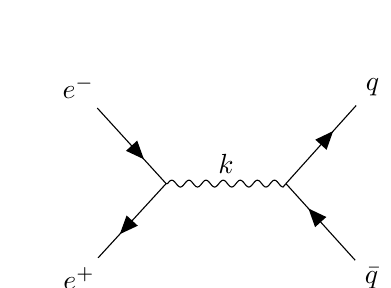
\begin{tikzpicture}[baseline={(0,0.5)}]
        \feynmandiagram [horizontal=a to b] {
        i1 [particle=\(e^{+}\)] -- [anti fermion] a -- [anti fermion] i2 [particle=\(e^{-}\)],
        a -- [photon, edge label=\(k\)] b,
        f1 [particle=\(q\)] -- [anti fermion] b -- [anti fermion] f2 [particle=\(\bar{q}\)],
        };            
        \end{tikzpicture}}\\
        \\
        &= (-ie)\bar{v}(p_2)\gamma^\mu u(p_1) \frac{-ig_{\mu\nu}}{k^2}(-ieQ_f)\bar{u}(p_3)\gamma^\nu v(p_4)\\
        &= -i\frac{(-ie)^2Q_f}{s}\bar{v}(p_2)\gamma^\mu u(p_1) \bar{u}(p_3)\gamma_\mu v(p_4).
        \label{EQ. eemm}
    \end{aligned}
\end{equation}
Taking the hermitian conjugate of $\mathcal{M}_0$, we find
\begin{equation}
    \mathcal{M}_0^\dagger = \frac{e^2Q_f}{s}\bar{u}(p_1)\gamma^\mu v(p_2) \bar{v}(p_4)\gamma_\mu u(p_3).
\end{equation}
One should notice that in the above calculation, we have made the colour implicit. Since we do not measure the colour of the quarks, we should sum over the colours. Therefore, by averaging over the incoming spins and summing over the outgoing spins and colours, we have  
\begin{equation}
    \begin{aligned}
        \frac{1}{4}\sum_\text{spins, colours}\mathcal{M}_0\mathcal{M}_0^\dagger &=  \sum_\text{spins, colours}\frac{e^4Q_f^2}{4s^2}[\bar{u}(p_1)\gamma^\nu v(p_2)][\bar{v}(p_2)\gamma^\mu u(p_1)] [\bar{u}_i(p_3)\gamma_\mu v_i(p_4)][\bar{v}_i(p_4)\gamma_\nu u_i(p_3)]\\
        &= \frac{3e^4Q_f^2}{4s^2}\Tr{\slashed{p}_1 \gamma^\nu \slashed{p}_2 \gamma^\mu} \Tr{\slashed{p}_3 \gamma_\mu \slashed{p}_4 \gamma_\nu}\\
        &= 3\frac{4e^4Q_f^2}{s^2} (p_1^\nu p_2^\mu - p_{12}g^{\mu\nu} + p_1^\mu p_2^\nu)(p_3^\nu p_4^\mu - p_{34}g^{\mu\nu} + p_3^\mu p_4^\nu)\\
        &= 3\frac{4e^4Q_f^2}{s^2}(2p_{13}p_{24} + 2p_{14}p_{23})\\
        &= 3\frac{2e^4Q_f^2}{s^2}(t^2+u^2).
    \end{aligned}
\end{equation}
In the centre of mass frame, we have
\begin{equation}
    p_1 = (E, 0, 0, E), \quad p_2 = (E, 0, 0, -E), \quad p_3 = (E, E\sin\theta, 0, E\cos\theta), \quad p_4 (E, -E\sin\theta, 0, -E\cos\theta),
\end{equation}
which implies 
\begin{equation}
    t =  -2p_{13} = -2E^2(1-\cos\theta), \quad u = -2p_{14} = -2E^2(1+\cos\theta).
\end{equation}
Thus, the differential corss section becomes
\begin{equation}
\begin{aligned}
    \frac{d\sigma}{d\Omega} &= \frac{3e^4Q_f^2}{32\pi^2s^3}\left(\frac{s^2}{4}(1-\cos\theta)^2 + \frac{s^2}{4}(1+\cos\theta)^2\right)\\
    &= \frac{3\alpha^2Q_f^2}{4s}(1+\cos^2\theta).
\end{aligned}
\end{equation}
Then,
\begin{equation}
\begin{aligned}
        \sigma(e^+e^-\to\bar{q}q) &= 2\pi\frac{3\alpha^2Q_f^2}{4s}\int^1_{-1}d(\cos\theta)(1+\cos^2\theta)\\
        &= \frac{4\alpha^2\pi}{3s}\cdot 3Q_f^2.
\end{aligned}
\end{equation}

Now, let us consider the diagram involving one virtual gluon, which is the diagram
\begin{equation}
\begin{aligned}
i\delta\mathcal{M} &={
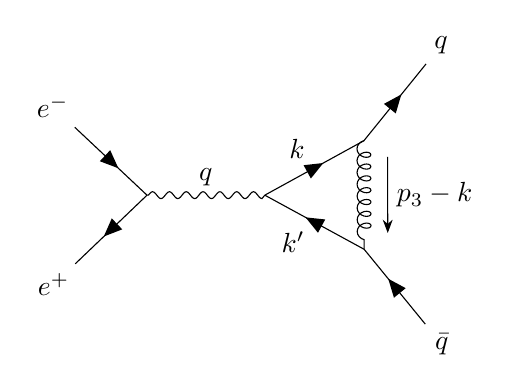
\begin{tikzpicture}[baseline={(0,-1.1)}]
  \begin{feynman}
    \diagram[horizontal=a to b]{
      % incoming leptons: e- from left, e+ from right
      i1 [particle=\(e^{-}\)] -- [fermion] a -- [fermion] i2 [particle=\(e^{+}\)],
      % s-channel photon
      a -- [photon, edge label=\(q\)] b,
      % outgoing antiquark on left, quark on right
      f2 [particle=\(\bar q\)] -- [fermion] v2 -- [fermion, edge label=$k'$] b -- [fermion, edge label=$k$] v1 -- [fermion] f1 [particle=\(q\)],
      % virtual gluon between them
      v1 -- [gluon, momentum=$p_3-k$] v2,
    };
  \end{feynman}
\end{tikzpicture}}\\[6pt]
&= (-ie)\,\bar v(p_2)\gamma^\mu u(p_1)\;\frac{-ig_{\mu\nu}}{k^2}\;(-ieQ_f)\,
   \Big[\bar u(p_3)\,\delta\Gamma^\nu(p_3,p_4)\,v(p_4)\Big] \\
&= \frac{(-ie)^2 Q_f}{s}\,\bar v(p_2)\gamma^\mu u(p_1)\,
   \Big[\bar u(p_3)\,\delta\Gamma_\mu(p_3,p_4)\,v(p_4)\Big].
\label{EQ. eemm}
\end{aligned}
\end{equation}

We shall focus on evaluating $\bar u(p_3)\,\delta\Gamma_\mu(p_3,p_4)\,v(p_4)$, which gives
\begin{equation}
    \begin{aligned}
        \bar u(p_3)\,\delta\Gamma_\mu(p_3,p_4)\,v(p_4) &= (-ig)^2\int \frac{d^4k}{(2\pi)^4}\bar{u}(p_3)\gamma^\alpha\frac{i\slashed{k}}{k^2 + i\varepsilon}\gamma_\mu\frac{i\slashed{k'}}{k'^2+i\varepsilon}\gamma^\beta v(p_4)\frac{-ig_{\alpha\beta}}{(p_3-k)^2-\mu^2+i\varepsilon}\\
        &= -ig^2\int \frac{d^4k}{(2\pi)^4}\bar{u}(p_3)\frac{\gamma^\alpha\slashed{k}\gamma_\mu\slashed{k'}\gamma_\alpha}{(k^2+i\varepsilon)(k'^2+i\varepsilon)((p_3-k)^2-\mu^2+i\varepsilon)}v(p_4)\\
        & = 2ig^2\int \frac{d^4k}{(2\pi)^4}\bar{u}(p_3)\frac{\slashed{k'}\gamma_\mu\slashed{k}}{(k^2+i\varepsilon)(k'^2+i\varepsilon)((p_3-k)^2-\mu^2+i\varepsilon)}v(p_4).
    \end{aligned}
\end{equation}

Now, we can simplify this using the Feynman parameters:
\begin{equation}
    \frac{1}{ABC} = \int^1_0dxdydz\delta(x+y+z-1)\frac{2}{(xA+yB+zC)^3} = \int^1_0dxdydz\delta(x+y+z-1)\frac{2}{D^3}.
\end{equation}
Thus, the denominator of becomes
\begin{equation}
\begin{aligned}
    D  &= z(k^2+i\varepsilon) + y(k'^2+i\varepsilon)+ z((p_3-k)^2-\mu^2+i\varepsilon) \\
    &= k^2 + yq^2 -2k\cdot (yq + zp_3)- z\mu^2 + i\varepsilon\\
    &= (k-(yq+zp_3))^2 - (yq+zp_3)^2 + yq^2- z\mu^2 + i\varepsilon\\
    &= (k-(yq+zp_3))^2 - 2zyq\cdot p_3 + y(1-y)q^2- z\mu^2 + i\varepsilon\\
    &= (k-(yq+zp_3))^2 + zy(q-p_3)^2 -zyq^2 + y(1-y)q^2- z\mu^2 + i\varepsilon\\
    &= (k-(yq+zp_3))^2  + y(1-y-z)q^2- z\mu^2 + i\varepsilon,
\end{aligned}
\end{equation}
where we have used $k' = k-q$ and $x+y+z=1$. Now, substitute $l = k-yq-zp_3$, we find
\begin{equation}
    D = l^2 - \Delta + i\varepsilon,
\end{equation}
where
\begin{equation}
    \Delta \equiv - xyq^2 + z\mu^2.
\end{equation}
The numerator, $N^\mu$, now becomes
\begin{equation}
    \begin{aligned}
        N_\mu &= \bar{u}(p_3)(\slashed{q} - \slashed{l}-y\slashed{q}-z\slashed{p}_3)\gamma_\mu(\slashed{l}+y\slashed{q}+z\slashed{p}_3)v(p_4)\\
        &= \bar{u}(p_3)((1-y)\slashed{q} - \slashed{l})\gamma_\mu(\slashed{l}+y\slashed{q}+z\slashed{p}_3)v(p_4)\\
        &= \bar{u}(p_3)((1-y)\slashed{q} - \slashed{l})[(-\slashed{l}-y\slashed{q}-z\slashed{p}_3)\gamma_\mu + 2l_\mu + 2yq_\mu + 2zp_{3\mu}]v(p_4).
    \end{aligned}
\end{equation}
Recall that the integral involving only one $l^\mu$ vanishes:
\begin{equation}
    \int \frac{d^4l}{(2\pi)^4}\frac{l^\mu}{D^3} = 0.
\end{equation}
Also, recall
\begin{equation}
    \int \frac{d^4l}{(2\pi)^4}\frac{l^\mu l^\nu}{D^3} = \int \frac{d^4l}{(2\pi)^4}\frac{\frac{1}{4}g^{\mu\nu}l^2}{D^3}
\end{equation}
Thus, the above becomes
\begin{equation}
    \begin{aligned}
        N_\mu &\to \bar{u}(p_3)[(-y(1-y)q^2 + -2z(1-y)q\cdot p_3 + l^2 )\gamma_\mu - \frac{1}{2}l^2\gamma_\mu]v(p_4) \\
        &= \bar{u}(p_3)[(-y(1-y)q^2 + z(1-y)(q+p_3)^2 - z(1-y)q^2 + l^2 )\gamma_\mu - \frac{1}{2}l^2\gamma_\mu]v(p_4)\\
        &= \bar{u}(p_3)(-(y+z)(1-y)q^2  + \frac{1}{2}l^2 )\gamma_\mu v(p_4).
    \end{aligned}
\end{equation}
Thus, we see that the 1-loop correction is of the form 
\begin{equation}
    i\delta\mathcal{M} = i\mathcal{M}_0 \frac{\delta F_1(q^2)}{Q_f^2},
\end{equation}
where 
\begin{equation}
    \delta F_1(q^2) = 4ig^2Q_f^2\int^1_0dxdydz\int\frac{d^4l}{(2\pi)^4}\frac{-(y+z)(1-y)q^2  + \frac{1}{2}l^2}{D^3}\delta(x+y+z-1).
\end{equation}
Thus, our job now simplifies to evaluate $\delta F_1(q^2)$ and since it describes the modification of electric charge, we can then simply plug $F_1(q^2)$ instead of $Q_f$ into the cross section, which gives
\begin{equation}
    \sigma(e^+e^-\to\bar{q}q) = \frac{4\alpha^2\pi}{3s}\cdot 3\abs{F_1(s)}^2
\end{equation}
with 
\begin{equation}
    F_1(q^2) = Q_f^2 + \delta F_1(q^2)
\end{equation}
to first order of $\alpha_g$.

Now, using Pauli-Villars regularization and Wick's rotation, we have
\begin{equation}
    \delta F_1(q^2) = \frac{\alpha_gQ_f^2}{2\pi} \int^1_0 dxdydz \left\{\ln\left(\frac{z\Lambda^2}{\Delta}\right) + \frac{(y+z)(1-y)q^2}{- xyq^2 + z\mu^2}\right\}\delta(x+y+z-1).
\end{equation}

On the other hand, to maintain the condition $F_1(0)= Q_f^2$, we should renormalize $\delta F_1(q^2)$ to be
\begin{equation}
    \delta F_1(q^2) - \delta F_1(0).
\end{equation}

Thus, the integral becomes
\begin{equation}
    \delta F_1(q^2) = \frac{\alpha_gQ_f^2}{2\pi} \int^1_0 dxdydz \left\{\ln\left(\frac{z\mu^2}{- xyq^2 + z\mu^2}\right) + \frac{(y+z)(1-y)q^2}{- xyq^2 + z\mu^2}\right\}\delta(x+y+z-1).
\end{equation}
\newpage
\textbf{(b)} Before we continue to compute the integral above, let us study the process of $e^-e^+ \to \bar{q}qg$. Let $q$ be the total 4-momentum of the process and $k_1,k_2,k_3$ be the 4-momentum of the quark, antiquark and the gluon, respectively. 

The Lorentz-invariant phase space integral is given by
\begin{equation}
    \int d\Pi_3 = (2\pi)^4\int \frac{d^3k_1}{(2\pi)^3}\frac{1}{2E_1}\frac{d^3k_2}{(2\pi)^3}\frac{1}{2E_2}\frac{d^3k_3}{(2\pi)^3}\frac{1}{2E_3}\delta^4(k_1+k_2+k_3-q).
\end{equation}

It is convenient to define $x_i$ as
\begin{equation}
    x_i = \frac{2k_i\cdot q}{q^2}.
\end{equation}
In the centre of mass frame,
\begin{equation}
    q = (E_\text{CM},0,0,0), \quad k_i = (E_i, \vec{k}_i).
\end{equation}
Thus, 
\begin{equation}
    x_i = \frac{2E_i}{E_\text{CM}},
\end{equation}
which is the ratio between the particle in the centre of mass frame to the total centre of mass energy.

\textbf{(i)} 
\begin{equation}
    \sum_ix_i = \frac{2\sum_ik_i\cdot q}{q^2} = 2.
\end{equation}
\textbf{(ii)} Now, we need to show that all the Lorentz scalars involving only the final state momenta can be expressed in terms of $x_i$. We only need to consider
\begin{equation}
    (k_1+k_2)^2 = (q-k_3)^2 = q^2 - q^2x_3 + m_3^2 =q^2(1-x_3) + m_3^2.
\end{equation}
The same thing applies to other combinations of $k_i$.

\textbf{(iii)} Now, we are ready to evaluate the phase space integral:
\begin{equation}
    \begin{aligned}
        \int d\Pi_3&= (2\pi)^4\int\frac{d^3k_1d^3k_2}{(2\pi)^92E_12E_22E_3}\delta(E_1+E_2+E_3-E_\text{CM})\bigg|_{\vec{k}_3 = -\vec{k}_1-\vec{k}_2}
    \end{aligned}
\end{equation}
The integral measure can be written as 
\begin{equation}
    d^3k_1d^3k_2 = k_1^2k_2^2dk_1dk_2d\Omega_1d\Omega_{12}
\end{equation}
with a slight ambiguity of notations (from now on we use $k_1=\abs{\vec{k}_1}$). $\Omega_1$ is the solid angle between $\vec{k}_1$ and $\vec{q}$ and $\Omega_{12}$ is the solid angle between $\vec{k}_1$ and $\vec{k}_2$. The delta function can be written as 
\begin{equation}
\begin{aligned}
    \delta(E_1+E_2+E_3-E_\text{CM}) &= \delta\left(E_1+E_2+\sqrt{\mu^2+(\vec{k}_1+\vec{k}_2)^2}-E_\text{CM}\right)\\
    &= \delta\left(\sqrt{\mu^2+k_1^2+k_2^2+2k_1k_2\cos\theta_{12}}-(E_\text{CM}-E_1-E_2)\right)\\
    &= \frac{E_3}{k_1k_2} \delta\left( \cos\theta_{12} - \frac{E_3^2-k_1^2-k_2^2-\mu^2}{2k_1k_2} \right).
\end{aligned}
\end{equation}

Thus, the integral becomes
\begin{equation}
    \begin{aligned}
        \int d\Pi_3&=\frac{2(2\pi)^2}{(2\pi)^5} \int^\infty_0dk_1dk_2\frac{k_1^2k_2^2}{2k_12k_22E_3}\int^1_{-1}d(\cos\theta_{12})\frac{E_3}{k_1k_2} \delta\left( \cos\theta_{12} - \frac{E_3^2-k_1^2-k_2^2-\mu^2}{2k_1k_2} \right)\\
        &= \frac{1}{32\pi^3}\int dk_1dk_2\\
        &= \frac{1}{32\pi^3}\int dE_1dE_2.
    \end{aligned}
\end{equation}
Recall, in the centre of mass frame, we have 
\begin{equation}
    x_i = \frac{2E_i}{E_\text{CM}} \implies dx_i = \frac{2}{E_\text{CM}}dE_i.
\end{equation}
Therefore, the integral simplifies to 
\begin{equation}
    \int d\Pi_3 = \frac{q^2}{128\pi^3}\int dx_1dx_2.
\end{equation}

Now, let us find the region of integration. The integration variables are bounded by the curves
\begin{equation}
    E_\text{CM} = E_1 + E_2 + \sqrt{\mu^2 + (E_1+E_2)^2}, \quad \text{or} \quad E_\text{CM} = E_1 + E_2 + \sqrt{\mu^2 + (E_1-E_2)^2},
\end{equation}
which implies
\begin{equation}
    \begin{cases}
        E_\text{CM}^2 - 2E_\text{CM}(E_1+E_2)-2E_1E_2 = \mu^2 + 2E_1E_2\\
        E_\text{CM}^2 - 2E_\text{CM}(E_1+E_2)-2E_1E_2 = \mu^2  -2E_1E_2
    \end{cases} 
    \implies
    \begin{cases}
        (1-x_1)(1-x_2) =\mu^2/s\\
        x_1+x_2 = 1-\mu^2/s.
    \end{cases}
\end{equation}
Thus, the integral is bounded by these two curves. Specifically, $x_1$ is bounded by
\begin{equation}
\begin{aligned}
    &(1-x_1)(\frac{\mu^2}{s}+x_1) = \frac{\mu^2}{s} \\
    \implies & x_1^2-\left(1-\frac{\mu^2}{s}\right)x_1 = 0 \\
    \implies & x_1 = 1-\frac{\mu^2}{s}\\
    \implies &0<x_1 < 1 - \frac{\mu^2}{s}.
\end{aligned}
\end{equation}
Then, the boundary of $x_2$ can be found with simple algebra:
\begin{equation}
    \begin{aligned}
        &\begin{cases}
        x_2 = 1-\frac{\mu^2/s}{1-x_1}\\
        x_2 = 1-x_1-\frac{\mu^2}{s}
    \end{cases} \\
        \implies & 
        1-x_1-\frac{\mu^2}{s} < x_2 <1-\frac{\mu^2}{s(1-x_1)}.
    \end{aligned}
\end{equation}


\textbf{(c)} Now, let us consider the diagrams contributing to the process $e^+e^-\to\bar{q}qg$ of the leading order of $\alpha$ and $\alpha_g$. The two diagrams are
\begin{equation}
\begin{aligned}
i\mathcal{M} &=
% ----------------- (A) Gluon emission from quark (quark on top) -----------------
{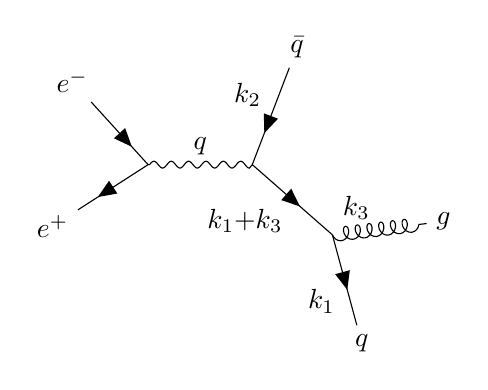
\begin{tikzpicture}[baseline={(0,0.8)}]
  \begin{feynman}
    \diagram[horizontal=a to b]{
      % incoming leptons
      i1 [particle={$e^{+}$}] -- [anti fermion] a -- [anti fermion] i2 [particle={$e^{-}$}],
      % s-channel photon
      a -- [photon, edge label={\(q\)}] b,
      % final state: quark on top, antiquark on bottom
      b -- [fermion, edge label'={$k_1{+}k_3$}] v1 -- [fermion, edge label'={$k_1$}] f1 [particle={$q$}],
      b -- [anti fermion, edge label={$k_2$}] f2 [particle={$\bar q$}],
      % gluon from quark line (top)
      v1 -- [gluon, edge label={$k_3$}] g1 [particle={$g$}],
    };
  \end{feynman}
\end{tikzpicture}}
\;+\;
% ----------------- (B) Gluon emission from antiquark (antiquark on top) ----------
{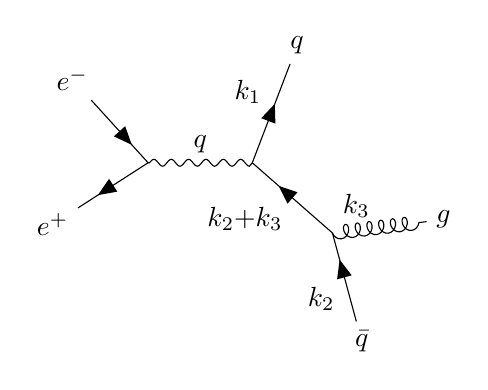
\begin{tikzpicture}[baseline={(0,0.8)}]
  \begin{feynman}
    \diagram[horizontal=a to b]{
      % incoming leptons
      i1 [particle={$e^{+}$}] -- [anti fermion] a -- [anti fermion] i2 [particle={$e^{-}$}],
      % s-channel photon
      a -- [photon, edge label={\(q\)}] b,
      % final state: antiquark on top, quark on bottom
      b -- [anti fermion, edge label'={$k_2{+}k_3$}] v2 -- [anti fermion, edge label'={$k_2$}] f2 [particle={$\bar q$}],
      b -- [fermion, edge label={$k_1$}] f1 [particle={$q$}],
      % gluon from antiquark line (top)
      v2 -- [gluon, edge label={$k_3$}] g2 [particle={$g$}],
    };
  \end{feynman}
\end{tikzpicture}}\\
&= \frac{-ig_{\mu\nu}}{q^2+i\varepsilon}\bar{v}(p_2)(-ie)\gamma^\mu u(p_1)\bar{u}(k_1)(-ig)\gamma^\alpha\frac{i(\slashed{k}_2 + \slashed{k}_3)}{(k_2+k_3)^2+ i\varepsilon}(-ieQ_f)\gamma^\nu v(k_2)\epsilon_\alpha^*(k_3) \\
&\qquad - \frac{-ig_{\mu\nu}}{q^2+i\varepsilon}\bar{v}(p_2)(-ie)\gamma^\mu u(p_1)\bar{u}(k_1)(-ieQ_f)\gamma^\nu \frac{i(\slashed{k}_1 + \slashed{k}_3)}{(k_1+k_3)^2+ i\varepsilon}(-ig)\gamma^\alpha v(k_2)\epsilon_\alpha^*(k_3)\\
&= \frac{ie^2g Q_f}{s}\bar{v}(p_2)\gamma^\mu u(p_1)\bar{u}(k_1)\left[\gamma^\alpha\frac{(\slashed{k}_2 + \slashed{k}_3)}{(k_2+k_3)^2+ i\varepsilon}\gamma_\mu - \gamma_\mu\frac{(\slashed{k}_1 + \slashed{k}_3)}{(k_1+k_3)^2+ i\varepsilon}\gamma^\alpha \right]v(k_2)\epsilon_\alpha^*(k_3),
\end{aligned}
\end{equation}
while the minus sign arises from the anticommutation relation between fermions. This can be seen by writing down the contractions individually.

Then, summing over the spins, colours and polarisations, we have
\begin{equation}
    \begin{aligned}
        \frac{1}{4}\sum_\text{s,c,p}\abs{\mathcal{M}}^2 &= \frac{3e^4g^2Q_f^2}{4s^2}\Tr[\slashed{p}_2\gamma^\mu\slashed{p}_1\gamma^\nu]\Tr\bigg\{\slashed{k}_1\left[\gamma^\alpha\frac{(\slashed{k}_2 + \slashed{k}_3)}{(k_2+k_3)^2+ i\varepsilon}\gamma_\mu - \gamma_\mu\frac{(\slashed{k}_1 + \slashed{k}_3)}{(k_1+k_3)^2+ i\varepsilon}\gamma^\alpha \right]\slashed{k}_2\\
        &\qquad \qquad \qquad \qquad \qquad \qquad \qquad    \times\left[\gamma_\nu\frac{(\slashed{k}_2 + \slashed{k}_3)}{(k_2+k_3)^2+ i\varepsilon}\gamma^\beta - \gamma^\beta\frac{(\slashed{k}_1 + \slashed{k}_3)}{(k_1+k_3)^2+ i\varepsilon}\gamma_\nu \right]\bigg\}(-g_{\alpha\beta})\\
        &= -\frac{3e^4g^2Q_f^2}{4s^2}\Tr[\slashed{p}_2\gamma^\mu\slashed{p}_1\gamma^\nu]\bigg\{  \frac{1}{(k_2+k_3)^4}\Tr[\slashed{k}_1\gamma^\alpha(\slashed{k}_2 + \slashed{k}_3)\gamma_\mu\slashed{k}_2\gamma_\nu(\slashed{k}_2 + \slashed{k}_3)\gamma_\alpha]\\
        &\qquad \qquad \qquad \qquad \qquad \qquad+ \frac{1}{(k_1+k_3)^4}\Tr[\slashed{k}_1\gamma^\mu(\slashed{k}_1 + \slashed{k}_3)\gamma^\alpha\slashed{k}_2\gamma_\alpha(\slashed{k}_1 + \slashed{k}_3)\gamma_\nu]\\
        &\qquad \qquad \qquad \qquad \qquad \qquad- \frac{1}{(k_1+k_3)^2(k_2+k_3)^2}\Tr[\slashed{k}_1\gamma^\alpha(\slashed{k}_2 + \slashed{k}_3)\gamma_\mu\slashed{k}_2\gamma_\alpha(\slashed{k}_1 + \slashed{k}_3)\gamma_\nu]\\
        &\qquad \qquad \qquad \qquad \qquad \qquad - \frac{1}{(k_1+k_3)^2(k_2+k_3)^2}\Tr[\slashed{k}_1\gamma_\mu(\slashed{k}_1 + \slashed{k}_3)\gamma^\alpha\slashed{k}_2\gamma_\nu(\slashed{k}_2 + \slashed{k}_3)\gamma_\alpha]\bigg\}.
    \end{aligned}
\end{equation}
To proceed, let us simplify the calculation by throwing away the correlation between the initial beam axis and the direction of the final particles. To do that, consider the structure of the matrix element yielded above; we should have
\begin{equation}
    \int d\Pi_3 \frac{1}{4}\sum \abs{\mathcal{M}}^2 = L_{\mu\nu}\int d\Pi_3 H^{\mu\nu},
\end{equation}
where $L_{\mu\nu}$ is the electron trace and $H^{\mu\nu}$ is the quark trace. Now, if we integrate over all parameters of the final state except $x_1$ adn $x_2$, the only preferred 4-vector characterising the final state is $q^\mu.$ On the other hand, by Ward-Takahashi, we have (can be checked explicitly)
\begin{equation}
    q_\mu H^{\mu\nu}=0.
\end{equation}
Since, after integrating over final-state vectors, $\int H^{\mu\nu}$ is only dependent on scalars ($x_1$ and $x_2$) and $q^\mu$. Thus, it must take the form
\begin{equation}
    \int d\Pi_3 H^{\mu\nu} = \left(g^{\mu\nu} - \frac{q^\mu q^\nu}{q^2}\right)\cdot H，
\end{equation}
where $H$ is a scalar. The minus sign is there to preserve Ward identity. $H$ can be evaluated by contracting the above with $g_{\mu\nu}$:
\begin{equation}
    \int d\Pi_3 g_{\mu\nu}H^{\mu\nu} = 3H \implies H = \frac{1}{3}\int d\Pi_3 g_{\mu\nu}H^{\mu\nu}.
\end{equation}
Thus, 
\begin{equation}
    L_{\mu\nu}\int d\Pi_3 H^{\mu\nu} = L_{\mu\nu}\left(g^{\mu\nu} - \frac{q^\mu q^\nu}{q^2}\right)\frac{1}{3}\int d\Pi_3 g_{\rho\sigma}H^{\rho\sigma} = \frac{1}{3}L_{\mu\nu}g^{\mu\nu}\int d\Pi_3 g_{\rho\sigma}H^{\rho\sigma},
\end{equation}
where we have used the Ward identity once again.

Using this trick, we have
\begin{equation}
    \begin{aligned}
        \int d\Pi_3 \frac{1}{4}\sum \abs{\mathcal{M}}^2 &= -\frac{e^4g^2Q_f^2}{4s^2}\Tr[\slashed{p}_2\gamma^\mu\slashed{p}_1\gamma_\mu]\int d\Pi_3\bigg\{  \frac{1}{(k_2+k_3)^4}\Tr[\slashed{k}_1\gamma^\nu(\slashed{k}_2 + \slashed{k}_3)\gamma^\alpha\slashed{k}_2\gamma_\alpha(\slashed{k}_2 + \slashed{k}_3)\gamma_\nu]\\
        &\qquad \qquad \qquad \qquad \qquad \qquad+ \frac{1}{(k_1+k_3)^4}\Tr[\slashed{k}_1\gamma^\alpha(\slashed{k}_1 + \slashed{k}_3)\gamma^\alpha\slashed{k}_2\gamma_\nu(\slashed{k}_1 + \slashed{k}_3)\gamma_\alpha]\\
        &\qquad \qquad \qquad \qquad \qquad \qquad- \frac{1}{(k_1+k_3)^2(k_2+k_3)^2}\Tr[\slashed{k}_1\gamma^\alpha(\slashed{k}_2 + \slashed{k}_3)\gamma^\nu\slashed{k}_2\gamma_\alpha(\slashed{k}_1 + \slashed{k}_3)\gamma_\nu]\\
        &\qquad \qquad \qquad \qquad \qquad \qquad - \frac{1}{(k_1+k_3)^2(k_2+k_3)^2}\Tr[\slashed{k}_1\gamma^\nu(\slashed{k}_1 + \slashed{k}_3)\gamma^\alpha\slashed{k}_2\gamma_\nu(\slashed{k}_2 + \slashed{k}_3)\gamma_\alpha]\bigg\}.
    \end{aligned}
\end{equation}
Now, let us compute the traces:
\begin{equation}
    \begin{aligned}
        \Tr[\slashed{k}_1\gamma^\nu(\slashed{k}_2 + \slashed{k}_3)\gamma^\alpha\slashed{k}_2\gamma_\alpha(\slashed{k}_2 + \slashed{k}_3)\gamma_\nu] &= 4\Tr[\slashed{k}_1(\slashed{k}_2 + \slashed{k}_3)\slashed{k}_2(\slashed{k}_2 + \slashed{k}_3)]\\
        &= 16[2k_1\cdot(k_2+k_3)k_2\cdot(k_2+k_3)-k_{12}(k_2+k_3)^2]\\
        &= 16(2k_{13}k_{23}-\mu^2k_{12}).
    \end{aligned}
\end{equation}
and, similarly,
\begin{equation}
     \Tr[\slashed{k}_1\gamma^\nu(\slashed{k}_1 + \slashed{k}_3)\gamma^\alpha\slashed{k}_2\gamma_\alpha(\slashed{k}_1 + \slashed{k}_3)\gamma_\nu] =16(2k_{13}k_{23}-\mu^2k_{12}).
\end{equation}
At the limit $\mu\to 0$, we have
\begin{equation}
    16(2k_{13}k_{23}-\mu^2k_{12}) \to 8s^2(1-x_1)(1-x_2).
\end{equation}
On the other hand, the ``cross" traces gives
\begin{equation}
    \begin{aligned}
        &\Tr[\slashed{k}_1\gamma^\alpha(\slashed{k}_2 + \slashed{k}_3)\gamma^\nu\slashed{k}_2\gamma_\alpha(\slashed{k}_1 + \slashed{k}_3)\gamma_\nu]+ \Tr[\slashed{k}_1\gamma^\nu(\slashed{k}_1 + \slashed{k}_3)\gamma^\alpha\slashed{k}_2\gamma_\nu(\slashed{k}_2 + \slashed{k}_3)\gamma_\alpha] \\
        &= -128k_{12}(k_1+k_3)\cdot(k_2+k_3)\\
        &= -16[s(1-x_3)+\mu^2](\mu^2+s).
    \end{aligned}
\end{equation}
Under the massless limit, it becomes
\begin{equation}
    -16[s(1-x_3)+\mu^2](\mu^2+s) \to -16s^2(1-x_3).
\end{equation}
Then (under the massless limit), we find
\begin{equation}
    \begin{aligned}
        \int d\Pi_3 \frac{1}{4}\sum \abs{\mathcal{M}}^2 
        &= -\frac{e^4g^2Q_f^2}{4s^2}(-8p_{12})\int d\Pi_3\bigg\{\frac{32(1-x_1)}{(1-x_2)} + \frac{32(1-x_2)}{(1-x_1)} + \frac{64(1-x_3)}{(1-x_1)(1-x_2)}\bigg\}\\
        &=\frac{32e^4g^2Q_f^2}{s^2}\int d\Pi_3\frac{2-2(x_1+x_2+x_3)+x_1^2+x_2^2+2}{(1-x_1)(1-x_2)}\\
        &=\frac{32e^4g^2Q_f^2}{s}\int d\Pi_3\frac{x_1^2 + x_2^2}{(1-x_1)(1-x_2)}.
    \end{aligned}
\end{equation}
Thus, the differential cross section in the centre of mass frame is given by
\begin{equation}
    \begin{aligned}
        \frac{d\sigma(e^+e^-\to\bar{q}qg)}{dx_1dx_2} &= \frac{s}{128\pi^2}\frac{1}{2E_12E_2\abs{\vec{v}_{p_1}-\vec{v}_{p_2}}}\frac{32e^4g^2Q_f^2}{s}\frac{x_1^2 + x_2^2}{(1-x_1)(1-x_2)}\\
        &= (2\pi)^2(4\pi)\frac{s}{128\pi^2}\frac{16\alpha^2\alpha_gQ_f^2}{s^2}\frac{x_1^2 + x_2^2}{(1-x_1)(1-x_2)}\\
        &= \frac{2\pi\alpha^2\alpha_gQ_f}{s}\frac{x_1^2 + x_2^2}{(1-x_1)(1-x_2)}\\
        &= \frac{4\pi\alpha^2}{3s}\cdot 3Q_f \cdot \frac{\alpha_g}{2\pi}\frac{x_1^2 + x_2^2}{(1-x_1)(1-x_2)}.
    \end{aligned}
\end{equation}
\textbf{(d)} Now, we shall no longer work under the massless limit, but assuming $\mu^2 \ll s$. The averaged squared matrix element then takes the form
\begin{equation}
    \frac{1}{4}\sum\abs{\mathcal{M}}^2 = \frac{e^4g^2Q_f^2}{s}F(x_1,x_2,\mu^2/s),
\end{equation}
where
\begin{equation}
\begin{aligned}
        F(x_1,x_2,\mu^2/s) &= 4\left(\frac{1}{s^2(1-x_1)^2} + \frac{1}{s^2(1-x_2)^2}\right)\cdot 16\left(2\frac{[s(1-x_2)-\mu^2][s(1-x_1)-\mu^2]}{4} - \mu^2\frac{s(1-x_3)+\mu^2}{2}\right)\\
        &\qquad + 4\cdot16\frac{[s(1-x_3)+\mu^2](\mu^2+s)}{s^2(1-x_1)(1-x_2)}\\
        &= 32\left(\frac{1}{(1-x_1)^2} +\frac{1}{(1-x_2)^2}\right) \left([(1-x_2)-\mu^2/s][(1-x_1)-\mu^2/s] - (1-x_3)\mu^2/s+\mu^4/s^2\right)\\
        &\qquad + 64\frac{[x_1+x_2-1+\mu^2/s](\mu^2/s+1)}{(1-x_1)(1-x_2)}\\
        &=32\left(\frac{1}{(1-x_1)^2} +\frac{1}{(1-x_2)^2}\right) \left((1-x_2)(1-x_1) - \mu^2/s\right) + 64\frac{[x_1+x_2-1+\mu^2/s](\mu^2/s+1)}{(1-x_1)(1-x_2)}.
\end{aligned}
\end{equation}
Thus, we can redefine $F$ to be $F/32$, and then
\begin{equation}
    \frac{1}{4}\sum\abs{\mathcal{M}}^2 = \frac{32e^4g^2Q_f^2}{s}F(x_1,x_2,\mu^2/s)
\end{equation}
with
\begin{equation}
    F(x_1,x_2,\mu^2/s) = \left(\frac{1}{(1-x_1)^2} +\frac{1}{(1-x_2)^2}\right) \left((1-x_2)(1-x_1) - \mu^2/s\right) + 2\frac{[x_1+x_2-1+\mu^2/s](\mu^2/s+1)}{(1-x_1)(1-x_2)}.
\end{equation}
Now integrating over the region we defined in part (b):
\begin{equation}
    \begin{aligned}
        \int_0^{1-\mu^2/s} dx_1\int_{1-x_1-\mu^2/s}^{1-\frac{\mu^2}{s(1-x_1)}}dx_2 F(x_1,x_2,\mu^2/s)= 5 \;+\; 3 \ln(\alpha) \;+\; \ln^{2}(\alpha) \;-\; \tfrac{\pi^{2}}{3}
\;+\; \mathcal{O}(\alpha),
    \end{aligned}
 \end{equation}
 where we have used $\alpha= \mu^2/s$.
Thus, the cross section is given by 
\begin{equation}
    \sigma(e^+e^-\to \bar{q}qg) = \frac{4\pi\alpha^2}{3s}\cdot 3Q_f \cdot \frac{\alpha_g}{2\pi}\left[\; 5 + 3 \ln(\mu^2/s) + \ln^{2}(\mu^2/s) - \frac{\pi^{2}}{3}+ \mathcal{O}(\mu^2/s)\right].
\end{equation}

\textbf{(e)} Now, let us go back and evaluate the integral in part (a), again working in the limit $\mu^2\ll q^2 $:
\begin{equation}
    \begin{aligned}
        \delta F_1(q^2) &= \frac{\alpha_gQ_f^2}{2\pi} \int^1_0dz\int^{1-z}_0 dy\left[\ln{\frac{z\mu^2}{z\mu^2-y(1-y-z)q^2}}+\frac{(y+z)(1-y)q^2}{z\mu^2-(1-y-z)yq^2}\right].
    \end{aligned}
\end{equation}
Note that there are singularities in the region of integration. First, write $Q^2 =  -q^2$, and integrate for $Q^2>0$ (spacelike 4-momentum), which avoids the logarithm having a negative value in it. Thus, integral becomes
\begin{equation}
\begin{aligned}
        &\int^1_0dy\int^{1-y}_0 dz\left[\ln{\frac{z\mu^2}{z\mu^2+y(1-y-z)Q^2}}-\frac{(y+z)(1-y)Q^2}{z\mu^2+(1-y-z)yQ^2}\right]\\
        &=\int^1_0dy\frac{Q^2(-1+y)\left[(-1+y)(Q^2y+\mu^2)+ y(Q^2(1+y)-2\mu^2)\ln\frac{Q^2y}{\mu^2}\right]}{(-Q^2y+\mu^2)^2}\\
        &=
            \frac{1}{12 Q^{4}}\Bigg\{
            - (21 + 4\pi^{2}) Q^{4}
            + 4 (3 + 2\pi^{2}) Q^{2}\mu^{2}
            - 4\pi^{2}\mu^{4}\\
            &\quad + 12 \ln\!\left(\frac{Q}{\mu}\right)\Big[
            (3 - 4 i\pi) Q^{4}
            + 2(-1 + 4 i\pi) Q^{2}\mu^{2}
            - 4 i\pi \mu^{4}
            + 2(Q^{2} - \mu^{2})^{2} \ln\!\left(\frac{Q\mu}{Q^{2} - \mu^{2}}\right)
            \Big]\\
            &\quad + 12 (Q^{2} - \mu^{2})^{2} \operatorname{Li}_{2}\!\left(\frac{\mu^{2}}{Q^{2}}\right)
            \Bigg\}.
\end{aligned}
\end{equation}
This result is analytic. Thus, it can be generalised into the whole complex plane, including $Q^2 = -q^2-i\varepsilon$. Since we are concerned with the limit $\mu^2\ll q^2$, let us first take the limit $Q^2 \ll \mu^2$, then extend the result analytically Thus, 
\begin{equation}
    \begin{aligned}
        \delta F_1(Q^2) &= \frac{\alpha_g Q_f^{2}}{2\pi}\left[
                    -\frac{7}{4}
                    - \frac{\pi^{2}}{3}
                    - \frac{3}{2}\,\ln\!\left(\frac{\mu^{2}}{Q^{2}}\right)
                    + 2 i \pi \,\ln\!\left(\frac{\mu^{2}}{Q^{2}}\right)
                    - \frac{1}{2}\,\ln^{2}\!\left(\frac{\mu^{2}}{Q^{2}}\right) + \order{\frac{\mu^2}{Q^2}}\right].
    \end{aligned}
\end{equation}
Now, continue this result analytically to $Q^2 = -q^2-i\varepsilon$, the logrithm becoems
\begin{equation}
    \ln\frac{\mu^2}{Q^2} \to \ln \frac{\mu^2}{q^2} - i\pi.
\end{equation}
Thus, the form factor becomes
\begin{equation} 
    F_1(q^2) = Q_f^2 - \frac{\alpha_g}{4\pi}\left[
                    \ln^{2}\!\left(\frac{\mu^{2}}{q^{2}}\right)
                    + 3\,\ln\!\left(\frac{\mu^{2}}{q^{2}}\right)
                    + \frac{7}{2} - \frac{\pi^{2}}{3}
                    + 2 i \pi \,\ln\!\left(\frac{\mu^{2}}{q^{2}}\right)
                    + 3 i \pi \,\right].
\end{equation}
Since $F_1$ is the correction of electric charge, we can replace $Q_f^2$ in the cross section by it. Thus, we have
\begin{equation}
\begin{aligned}
    \sigma(e^+e^-\to\bar{q}q) &=\frac{4\alpha^2\pi}{3s}\cdot 3|F_1(q^2=s)|\\
    &=\frac{4\alpha^2\pi}{3s}\cdot 3Q_f^2\left[1 - \frac{\alpha_g}{2\pi}\left(\frac{7}{2}
                    - \frac{\pi^{2}}{3}
                    + 3\,\ln\!\left(\frac{\mu^{2}}{s}\right)
                    + \ln^{2}\!\left(\frac{\mu^{2}}{s}\right) + \order{\frac{\mu^2}{s}}\right)\right].
\end{aligned}
\end{equation}
\textbf{(e)} Putting the two cross sections together, one would note that all the infrared divergence term vanishes. Thus, we have
\begin{equation}
\boxed{
    \sigma(e^+e^- \to \bar{q}q \text{ or }\bar{q}qg) = \frac{4\alpha^2\pi}{3s}\cdot 3Q_f^2\left(1+\frac{3\alpha_g}{4\pi}\right).}
\end{equation}

\end{document}